\subsection{Impulse Response Coefficients}
\label{sec:Imp_res}
The Markov Parameters is determined on basis of the linearized state space model. In order to determine a state space model for the system, the SISO transfer functions determined in the previous paragraph is used. This yields the system in relation to the observer canonical form, which ensure the state space model to take the following form.
\begin{equation}
    \begin{gathered}
        \dot{x}(t)=A_{OC}\,x(t)+B_{OC}\,u(t) \\
        y(t) = C_{OC}\,x(t)+D_{OC}\,u(t)
    \end{gathered}
\end{equation}
The observer canonical form matrices is determined by the normalized transfer functions for the system. It was previously determined that there was no time delay in the system, so these are ignored in the analysis.\\
For $1^{st}$ order systems (normalized) the matrices are determined as follows:
\begin{equation}
    \frac{b_1\,s+b_0}{s+a_0}\xrightarrow{}
    A_{OC}=[-a_0] \quad 
    B_{OC}=[b_0-a_0\,b_1] \quad 
    C_{OC}=[1] \quad 
    D_{OC}=[b_1]
\end{equation}
For $2^{nd}$ order systems (normalized) the matrices are determined as follows
\begin{equation}
    \frac{b_2\,s^2+b_1\,s+b_0}{s^2+a_1\,s+a_0}\xrightarrow{}
    A_{OC}=\begin{bmatrix} -a_1 & 1 \\ -a_0 & 0 \end{bmatrix} \quad 
    B_{OC}=\begin{bmatrix} b_1-a_1\,b_2 \\ b_0-a_0\,b_2 \end{bmatrix} \quad 
    C_{OC}=\begin{bmatrix} 1 & 0 \end{bmatrix} \quad 
    D_{OC}=[b_2]
\end{equation}
The system is now discrtized according to the following:
\begin{equation}
    A_k=e^{A_{OC}\,T_s} \quad B_k=\int_0^{T_s}e^{A_{OC}\,t}\,B_{OC}\,dt \quad
    C_k=C_{OC} \quad
    D_k=D_{OC}
\end{equation}
The numerical values with a discretization time of $T_s=15$ is determined as:
\begin{equation}
    \begin{gathered}
        A_{k11}=[0.897] \qquad B_{k11}=[0.0215] \qquad C_{k11}=[1] \qquad D_{k11} = [0]\\
        A_{k12}=\begin{bmatrix} 0.7534 & 13.0837 \\ -0.0009 & 0.9926 \end{bmatrix} \qquad
        B_{k12}=\begin{bmatrix} 0.0013 \\ 0.0002 \end{bmatrix} \qquad
        C_{k12}=\begin{bmatrix} 1 & 0 \end{bmatrix} \qquad
        D_{k12} = [0]\\
        A_{k21}=\begin{bmatrix} 0.7518 & 13.0725 \\ -0.0011 & 0.9917 \end{bmatrix} \qquad
        B_{k21}=\begin{bmatrix} 0.9456 \\ 0.1377 \end{bmatrix} \qquad
        C_{k21}=\begin{bmatrix} 1 & 0 \end{bmatrix} \qquad
        D_{k21} = [0]\\
        A_{k22}=[0.9066] \qquad B_{k22}=[0.0256] \qquad C_{k22}=[1] \qquad D_{k22} = [0]\\
    \end{gathered}
\end{equation}
The response for the four transfer functions (SISO) is determined according to \cref{eq:SISO_markov}, and these can be used to determine the MIMO response according to \cref{eq:MIMO_markov}
\begin{equation}
    \begin{gathered}
        (H_0)_{i,j}=D_k\\
        (H_k)_{i,j}=C_k\,A^{k-1}_k\,B_k\quad k=1,2,\dots
    \end{gathered}
    \label{eq:SISO_markov}
\end{equation}
\begin{equation}
    H_k=
    \begin{bmatrix}
        (H_k)_{11} & (H_k)_{12}\\
        (H_k)_{21} & (H_k)_{22}
    \end{bmatrix}\quad k=1,2,\dots
    \label{eq:MIMO_markov}
\end{equation}
The MIMO response coefficients is used to generate the Hankel matrix as seen below.
\begin{equation}
    \mathcal{H}_{N,N}\triangleq
    \begin{bmatrix}
        H_1 & H_2 & \dots & H_N \\
        H_2 & H_3 & \dots & H_{N+1} \\
        \vdots & \vdots & \ddots & \vdots \\
        H_N & H_{N+1} & \dots & H_{2N-1}
    \end{bmatrix}
\end{equation}
It is known that the impulse reponse $(\mathcal{H}_i)^\infty_{i=1}$ has a minimal relization of order n, if and only if $\text{rank}(\mathcal{H}_{n+1,j})=\text{rank}(\mathcal{H}_{n,j})$. If this is true, it is possible to perform a Singular Value Decomposition (\textit{SVD}) of the Hankel matrix. For the given system, $n=3$ which yields the Hankel matrix to be the following:
\begin{equation}
    \mathcal{H}_{3,3}=\begin{bmatrix}
        0.0215 & 0.0013 & 0.0192 & 0.0033 & 0.0173 & 0.0049\\
        0.0009 & 0.0256 & 0.0025 & 0.0232 & 0.0037 & 0.0210\\
        0.0192 & 0.0033 & 0.0173 & 0.0049 & 0.0155 & 0.0060\\
        0.0025 & 0.0232 & 0.0037 & 0.0210 & 0.0045 & 0.0190\\
        0.0173 & 0.0049 & 0.0155 & 0.0060 & 0.0139 & 0.0067\\
        0.0037 & 0.0210 & 0.0045 & 0.0190 & 0.0050 & 0.0173
    \end{bmatrix}
\end{equation}
The \textit{SVD} is carried out on the above Hankel norm, which results in the following expression.
\begin{equation}
    \mathcal{H}_{N,N}=K\,\Lambda\,L^T=
    \begin{bmatrix}
        K_1 & K_2
    \end{bmatrix}\,
    \begin{bmatrix}
        \Lambda_1 & 0\\
        0 & 0
    \end{bmatrix}\,
    \begin{bmatrix}
        L_1 \\ L_2
    \end{bmatrix}
    = K_1\,\Lambda_1\,L_1^T
\end{equation}
The matrices $K_1$, $\Lambda_1$ and $L_1$ is determined with the inbuild \textit{SVD} function in \textit{MatLab} as seen below.
\begin{equation*}
    \begin{matrix}
        K_1=\begin{bmatrix}
            -0.3076 & 0.5710 & 0.4895 & -0.4599\\
            -0.5148 & -0.3830 & 0.5296 & 0.4291\\
            -0.3154 & 0.4748 & -0.0588 & 0.1053\\
            -0.4844 & -0.3017 & -0.0574 & -0.1151\\
            -0.3166 & 0.3941 & -0.4686 & 0.5600\\
            -0.4539 & -0.2355 & -0.5036 & -0.5161
        \end{bmatrix} &
        L_1=\begin{bmatrix}
            -0.3020 & 0.5717 & -0.4768 & 0.4793\\
            -0.5181 & -0.3821 & -0.5419 & -0.4063\\
            -0.3001 & 0.4835 & 0.0414 & -0.1263\\
            -0.4942 & -0.2867 & 0.0709 & 0.0931\\
            -0.2939 & 0.4089 & 0.4342 & -0.5841\\
            -0.4687 & -0.2097 & 0.5327 & 0.4892
        \end{bmatrix} \\
    \end{matrix}
\end{equation*}
\begin{equation}
    \Lambda_1=\begin{bmatrix}
    0.0712 & 0 & 0 & 0\\
    0 & 0.0458 & 0 & 0\\
    0 & 0 & 0.0004 & 0\\
    0 & 0 & 0 & 0.0001
    \end{bmatrix}
        \label{eq:K_L_Lambda}
\end{equation}
The Hankel matrix can also be described by the product of the extended observability matrix $\mathcal{O}_N$ and the extended controllability matrix $\mathcal{C}_N$ which is determined as seen below.
\begin{equation}
    \mathcal{O}_N=K_1\Lambda_1^{1/2} \qquad \mathcal{C}_N=\Lambda_1^{1/2}\,L_1^T
\end{equation}
Due to the fact that $K$, $L$, $K_1$ and $L_1$ are orthogonal matrices, it is possible to determine $B$ from the first $m$ columns of $\mathcal{C}_N$ and to determine $C$ from the first $p$ rows of $\mathcal{O}_N$. $D$ is determined on basis \cref{eq:SISO_markov}.
\begin{equation}
    \begin{gathered}
        B_k=(\mathcal{C}_N)_{(:,1:m)}=\Lambda_1^{1/2}\,\left((L_1)_{(1:m,:)}\right)^T=
        \begin{bmatrix}
            -0.0806 & -0.1382\\
            0.1224 & -0.0818\\
            -0.0098 & -0.0112\\
            0.0051 & -0.0043
        \end{bmatrix} \\
        C_k=(\mathcal{O}_N)_{(1:p,:)}=(K_1)_{(1:p,:)}\,\Lambda_1^{1/2}=
        \begin{bmatrix}
            -0.0821 & 0.1223 & 0.0101 & -0.0049\\
            -0.1374 & -0.0820 & 0.0109 & 0.0046
        \end{bmatrix}\\
        D_k=H_0=
        \begin{bmatrix}
            0 & 0 \\
            0 & 0
        \end{bmatrix}
    \end{gathered}
    \label{eq:Hankel_mat}
\end{equation}
In order to determine the $A$ matrix, the Hankel matrix is redefined according to the following:
\begin{equation}
    \Tilde{\mathcal{H}}_{(N+1,N+1)}=\mathcal{O}_N\,A_k\,\mathcal{C}_N
\end{equation}
The expression for $\mathcal{O}_N$ and $\mathcal{C}_N$ can is substitued, and then $A_k$ is isolated which yields:
\begin{equation}
    A_k=\Lambda_1^{-1/2}\,K_1^T\,\Tilde{H}_{(N+1,N+1)}\,L_1\,\Lambda_1^{-1/2}=
    \begin{bmatrix}
        0.9106 & -0.0302 & 0.1431 & 0.0106\\
        -0.0684 & 0.6638 & -0.0309 &  0.0951\\
        -0.1436 & 0.0283 & 0.5977 & -0.0353\\
        -0.0136 & -0.0943 & 0.0411 & 0.9010
   \end{bmatrix}
\end{equation}
With the above determine state space model it is now possible to determine the Markov parameters according to the below equation. The impulse response can be seen in \cref{fig:Markov}.
\begin{equation}
    \text{Markov parameters} = \begin{cases}
        D & i=0 \\
        C\,A^{i-1}\,B & i=1,2,...
    \end{cases}
    \label{eq:Markov}
\end{equation} 
\begin{figure}[H]
    \centering
    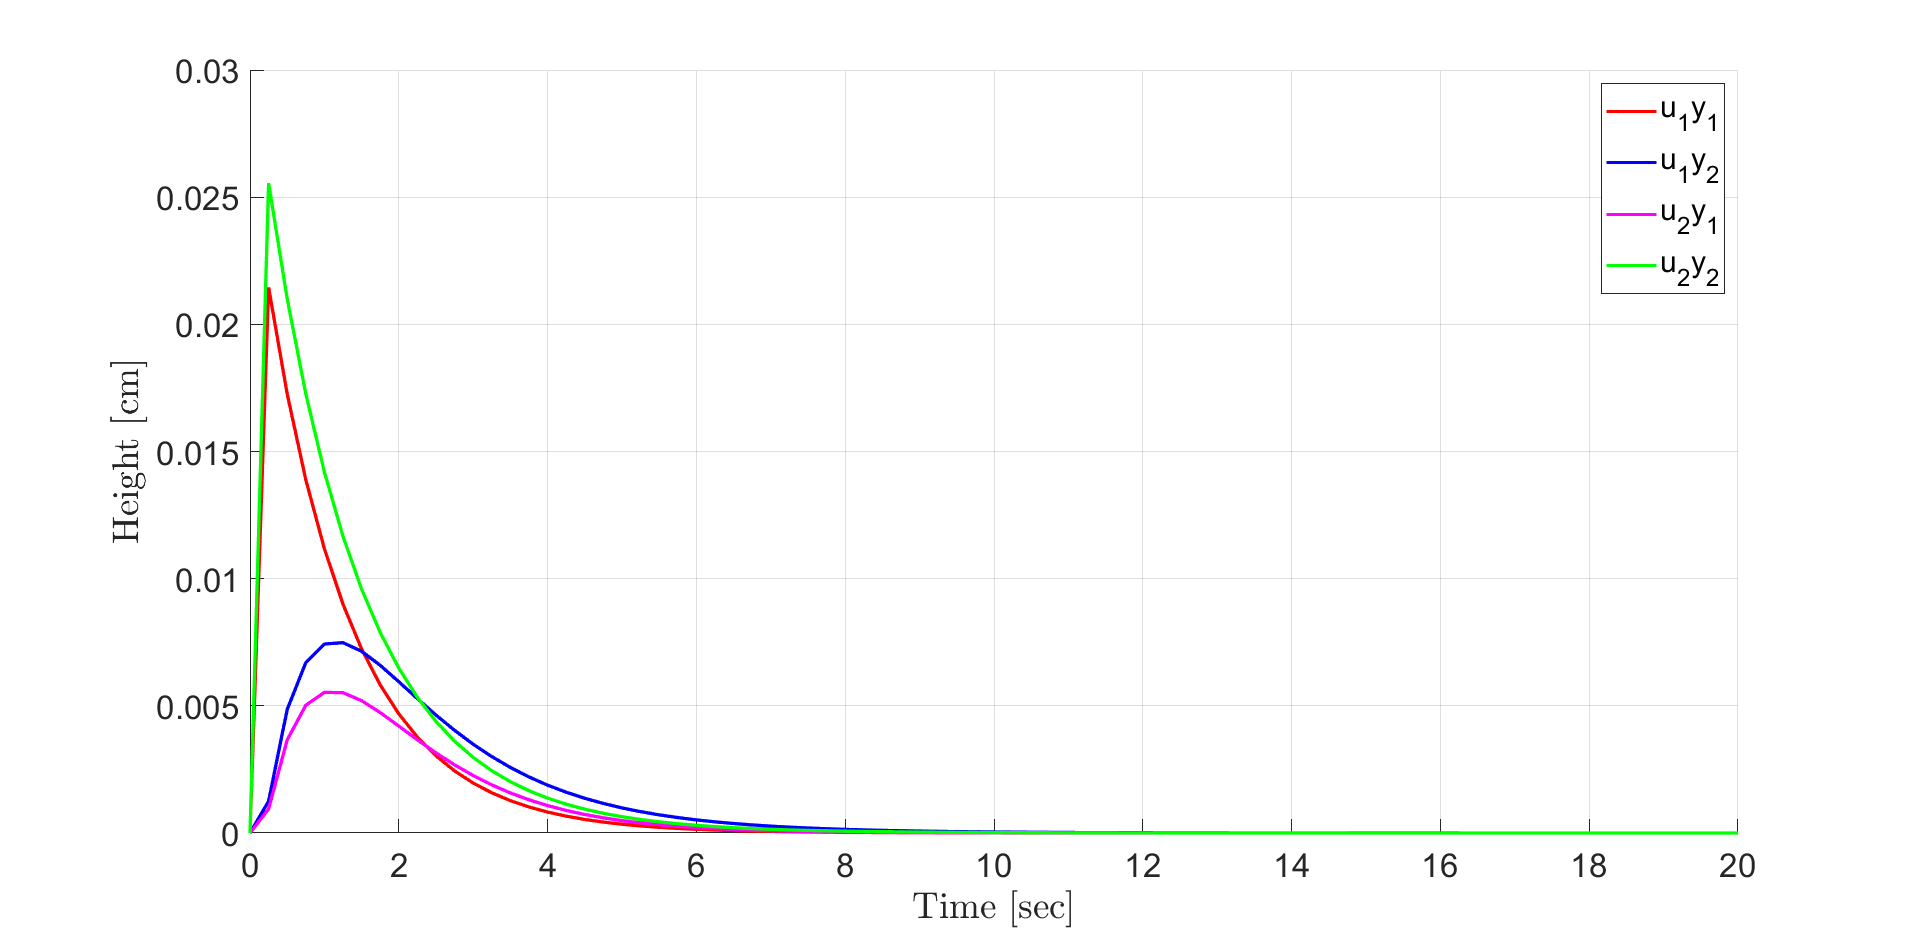
\includegraphics[width=1\textwidth]{Figures/Pr3.6_Markov.png}
    \caption{Impulse reponse}
    \label{fig:Markov}
\end{figure}